\chapter{Introduction}
\label{chap:intro}
\begin{itemize}
    \item A lot of data today ...
    \item Data analysis is an highly exploratory task
    \item Many processes to do the analysis, one example is the Knowledge Discovery in Databases (KDD) process (see \cref{fig:kdd}).
    \begin{figure}
        \centering
        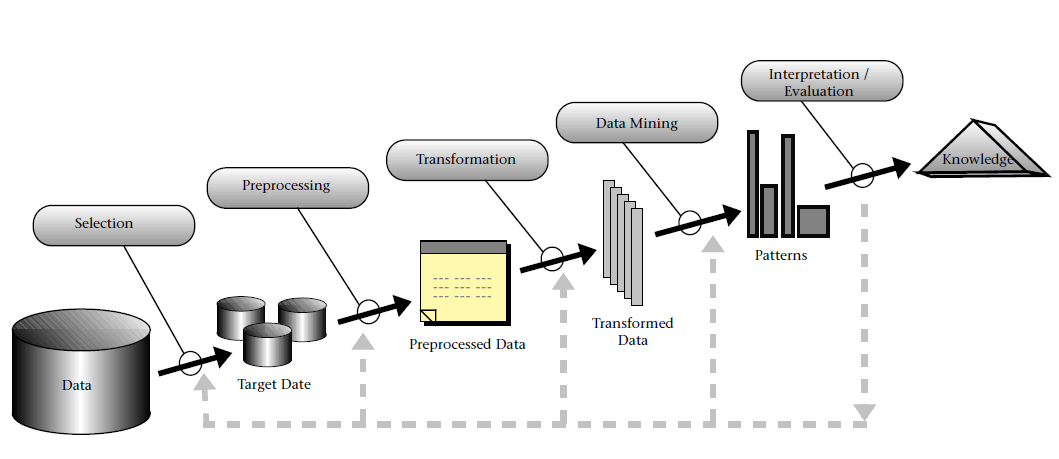
\includegraphics[width=\textwidth]{graphics/kdd_process.png}
        \caption{Overview of the KDD process \cite{Fayyad:1996:DMK:257938.257942}.}
        \label{fig:kdd}
    \end{figure}
    \item All process in common that iterative steps
    \item Focus of this work is in the data mining and evaluation step
    \item There are different steps involved here
    \item Important ones are the algorithm selection, the hyperparameter selection and the evaluation
    \item Human experts contribute to this steps by using their domain knowledge and experiences.
    \item Adjust parameters and algorithms. This is a trial-and-error process which takes a lot of time.
    \item  Also not always clear how to adjust parameters and algorithms.
    \item There are a lot of research in this area to help the analyst.
    One are so called \textit{White-box} methods.
    These methods aim at increasing the traceability by explaining the results of machine learning models to the analyst.
    Nevertheless, the choice of choosing an appropriate algorithm and its hyperparameters lies with the analyst.
    \item The other methods are \textit{Black-box} methods.
    In contrast to White-box methods, Black-box methods try to optimize machine learning models by automatically selecting an appropriate algorithm and its hyperparameters.
    But as the name suggest it is not clear what is happening inside this methods.
    The benefit of this methods is that they can be used without any expert knowledge and that they can lead to  higher accuracy and runtime savings compared to White-box methods.
    \item White-box = Human-in-the-loop
    \item Black-box = Take Human-out-of-the-loop
    \item Additionally, Black-box methods can be used without expert knowledge and still are able to achieve promising results.
    \item This research field is also known as \gls{AutoML}.
    Currently, there are a lot of \gls{AutoML} systems \todo{cite here the automl systems}.
    The general idea of this systems is shown in \cref{fig:automlWorkflow}.
    \begin{figure}
        \centering
        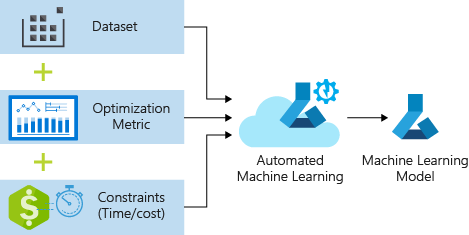
\includegraphics[width=0.5\textwidth]{graphics/flow_autom.png}
        \caption{Basic overview of the functionality of AutoML systems.}
        \label{fig:automlWorkflow}
    \end{figure}
    The inputs for the systems are three things: 
    \begin{itemize}
        \item The input datasets which have to be analyzed.
        \item A metric, according to which  the best model is searched.
        \item A constraint or budget, which can be for example a time budget of one hour.
        This means that the AutoML system terminates after one hour and returns the best model that was found in this time budget.
    \end{itemize}
    The input datasets, a metric, according to which the optimal model is searched and a constraint which  
    
    \item Some of this systems also learn from the performance of algorithms that were used in the past and transfer this knowledge to new unseen datasets, which is known as \textit{Meta-learning}.
    \item These systems do only cover supervised learning algorithms like classification.
    But many problems in Data Mining do not have the class label information.
    Hence, only unsupervised learning algorithms can be applied to this problems.
    Because of the missing class labels the concepts of the existing \gls{AutoML} systems cannot be applied directly.
    Therefore, for unsupervised learning there are only some approaches to use meta-learning but they all do not cover the combined problem of algorithm selection and hyperparameter optimization, which is known as \gls{CASH} problem.
    Also, they do not use the optimization methods to tune the hyperparameters that were used in the existing AutoML systems.
    \item Due to the limited work in this area, the goal of this work is to transfer these concepts of optimization methods and meta-learning on the unsupervised learning task clustering to solve the \gls{CASH} problem.
\end{itemize}
 The remainder of this paper is structured as follows ...
\xtodo{add this}